\documentclass[11pt]{article}
\usepackage{fullpage}
\usepackage{amsmath,amssymb}
\usepackage{graphicx}
\usepackage{color}
\usepackage[colorlinks,bookmarksopen,bookmarksnumbered,citecolor=red,urlcolor=red,breaklinks=true]{hyperref}
\newcommand{\cblue}[1]{{\color{blue}#1}}
\renewcommand{\vec}[1]{{#1}}
\newcommand{\note}[1]{\cblue{NOTE: #1}}
\title{Multilevel Monte Carlo for Quantum Field Theories on the Lattice}
\begin{document}
\maketitle
%%%%%%%%%%%%%%%%%%%%%%%%%%%%%%%%%%%%%%%%%%%%%%%%%%%%%%%%%%%%%%%%%%%%%%%%%%%%
\section{Challenge and Motivation}
%%%%%%%%%%%%%%%%%%%%%%%%%%%%%%%%%%%%%%%%%%%%%%%%%%%%%%%%%%%%%%%%%%%%%%%%%%%%
Quantum Field Theories (QFTs) \cite{Peskin1995}, such as Quantum Chromo Dynamics (QCD) predict fundamental properties of matter and are of paramount importance in High Energy Physics. If discretised on a space-time lattice, QCD allows first principles calculations of strongly interacting particles and is crucial for precise calculations, for example in New Physics predictions or to simulate the hadronic background in accelerators such as the Large Hadron Collider.
Using Feynman's Path Integral technique \cite{Feynman2010}, QFTs can be be formulated as statistical systems in $d=4$ space-time dimensions. Predictions of physical quantities are then calculated by generating a set of samples with Markov-Chain Monte Carlo Methods and evaluating the relevant quantity of interest on those samples. To obtain physically meaningful results, calculations need to be carried out for increasingly small lattice spacings $a$ and extrapolated to the continuum limit $a\rightarrow 0$. There are two key issues which make the accurate calculation challenging:
\begin{figure}
  \begin{center}
    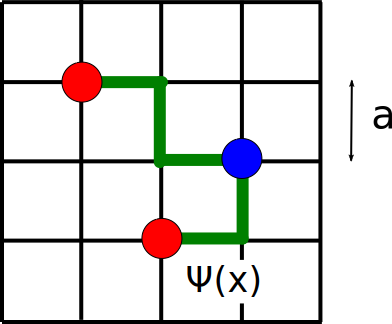
\includegraphics[width=0.3\linewidth]{lattice.pdf}
    \caption{Fields on a space-time lattice}
    \label{fig:lattice}
  \end{center}
\end{figure}
\begin{itemize}
\item Since the probability density is peaked around the classical trajectory, in the Metropolis-Hastings algorithm naively generated samples are highly correlated since the acceptance probability is small. This issue can be overcome by the Hybrid Monte Carlo method \cite{Duane1987}. However, the number of samples $N$ required to reduce the statistical sampling error below a tolerance $\epsilon$ still grows as $\mathcal{O}(\epsilon^{-2})$ due to fundamental law of large numbers. 
\item Since the number $M$ of lattice sites on a grid with spacing $a$ is $M \propto a^{-d}$, the cost to generate one sample grows as $\mathcal{O}(a^{-d})$. This already assumes that optimal algorithms are used when, for example, inverting large sparse matrices to calculate Fermion propagators. While if $3+1$ spacetime dimensions $d=4$, in some formulations (Domain Wall Fermions \cite{Kaplan1992}) the dimension of the system is even $d=5$.
\end{itemize}
If both the statistical and discretisation error (which we assume here to be linear in the lattice spacing) are to be reduced below a tolerance of $\epsilon\propto a$, the total cost of the method is $\mathcal{O}(\epsilon^{-(d+2)})$ where $d=4,5$. Together this leads to prohibitively high costs for Lattice QCD calculations which limit the range of available lattice spacings and extrapolations to the continuum limit.

In the following we explore Multilevel Monte Carlo sampling methods \cite{Heinrich2001,Giles2008,Giles2015}. As shown in \cite{Dodwell2015}, a Multilevel MCMC method has the potential to reduce the computational complexity from $\mathcal{O}(\epsilon^{-(d+2)})$ to $\mathcal{O}(\epsilon^2 |\log(\epsilon)|)$. Multilevel Monte Carlo uses a hierarchy of levels to construct an unbiased estimator. This requires calculation of the expectation value of differences between subsequent levels, which have a much smaller variance than the QoI itsself. An important requirement is that the theories used on two subsequent levels are ``close'', i.e. the coarse level theory should provide a good approximation for the coarse modes on the next-finer level. In QFT this can be achieved naturally by constructing the coarse theory as an effective theory of the fine-level model. While construction of the exact effective theory by integrating out the high-frequency modes is not possible (except in very simple cases), in many cases perturbation theory can be used to construct an approximate effective theory. In particular we expect this to be the case in QCD, which is asymptotically free. A whole machinery is available for carrying out perturbation theory on a lattice, see e.g. \cite{Rothe2005,Hart2009}.
%%%%%%%%%%%%%%%%%%%%%%%%%%%%%%%%%%%%%%%%%%%%%%%%%%%%%%%%%%%%%%%%%%%%%%%%%%%%
\section{Methods}
%%%%%%%%%%%%%%%%%%%%%%%%%%%%%%%%%%%%%%%%%%%%%%%%%%%%%%%%%%%%%%%%%%%%%%%%%%%%
To set the scene and introduce key concepts, we first discuss the much simpler case of quantum mechanics and show how it can be formulated as a statistical theory. Since this is effectively a one-dimensional field-theory, the gains are expected to be smaller here ($\mathcal{O}(\epsilon^{-3})\rightarrow\mathcal{O}(\epsilon^{-2}|\log(\epsilon)|)$). We discuss the generalisations required for the more interesting case of a $d$-dimensional Quantum Field Theory in Section \ref{sec:QFT}. 
%%%%%%%%%%%%%%%%%%%%%%%%%%%%%%%%%%%%%%%%%%%%%%%%%%%%%%%%%%%%%%%%%%%%%%%%%%%%
\subsection{Path integrals in Quantum Mechanics}
%%%%%%%%%%%%%%%%%%%%%%%%%%%%%%%%%%%%%%%%%%%%%%%%%%%%%%%%%%%%%%%%%%%%%%%%%%%%
Consider a particle of mass $m_0$ which moves in a potential $V(x)$ where $x(t)$ is the particle's position at time $t$.
Feynman's path integral \cite{Feynman2010} allows the calculation of the transition amplitude for starting at the point $x_i$ at time $t=0$ and ending at point $x_f$ at time $t=T$ as a sum over all possible paths $x(t)$ with $x(0)=x_i$,  $x(T)=x_f$, as shown in Fig. \ref{fig:path_integral} (left). This sum is denoted by $\int \mathcal{D}x(t)$. The crucial observation, exploited for example in \cite{Creutz1981}, is that by formulating the theory in imaginary time, the highly-oscillatory integrand is replaced by a real exponential and the path integral looks like a statistical system of temperature\footnote{In the ``zero-temperature'' limit quantum fluctuations disappear and only the classical trajectory contributes to the path integral.} $T\propto \hbar$.  The transition amplitude is given by
\begin{equation}
  \mathcal{A}(x_f\leftarrow x_i)=\langle x_f| e^{-HT} |x_i\rangle = \int\mathcal{D}x(t)\;e^{-S[x(t)]}.\label{eqn:path_integral_continuum}
\end{equation}
For simplicity we have chosen units in which Planck's constant $\hbar=1$.
For a given path $x(t)$ the action $S[x(t)]$ is
\begin{equation}
  S[x(t)] = \int_{0}^{T} \left(\frac{1}{2}m_0 \dot{x}(t)^2 + V(x(t))\right)\;dt
\end{equation}
\begin{figure}
  \begin{center}
    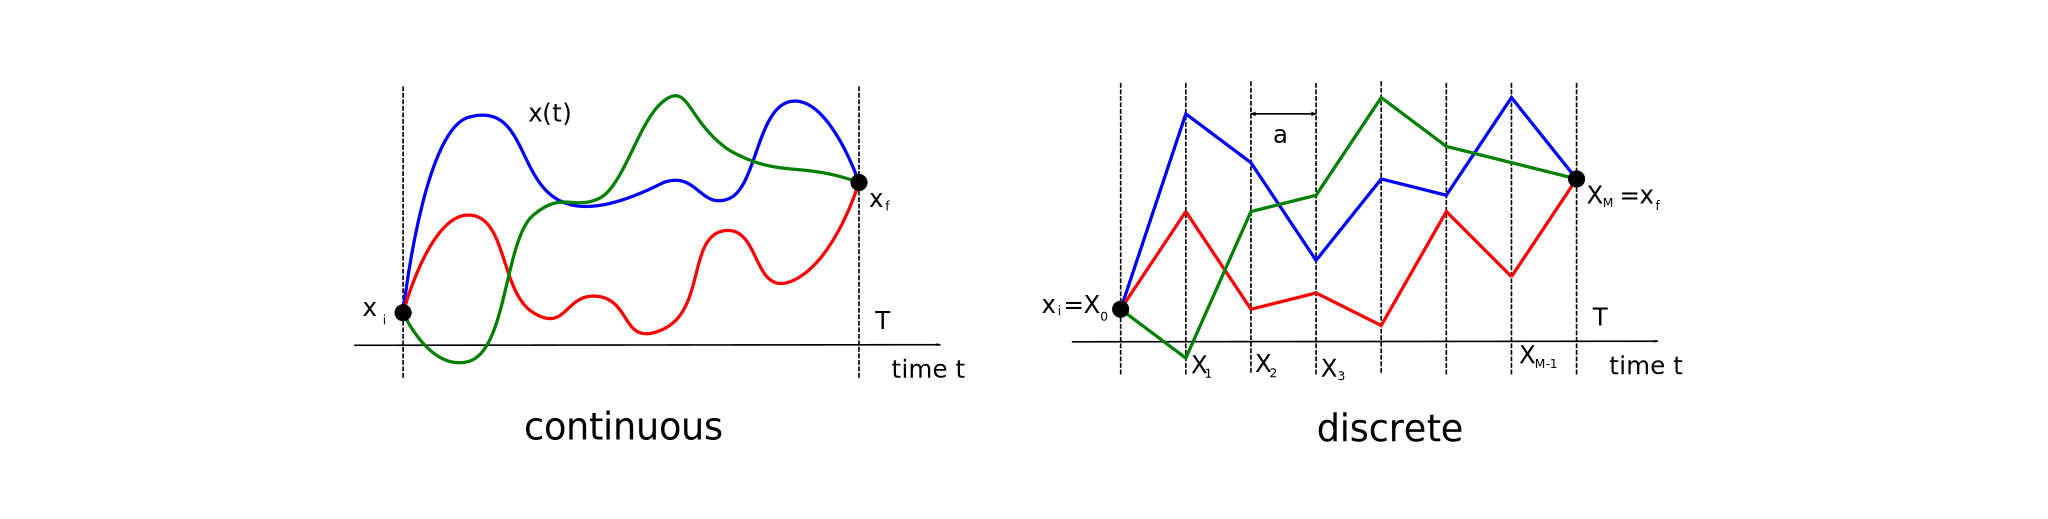
\includegraphics[width=\linewidth]{path_integral.pdf}
    \caption{Path integral in the continuum (left) and on a time-lattice of spacing $a$.}
    \label{fig:path_integral}
  \end{center}
\end{figure}
From now on we will also use periodic boundary conditions $x_i=x_f$ and integrate over $x_i$ as well in Eq. (\ref{eqn:path_integral_continuum}); in the infinite-volume limit $T\rightarrow \infty$ the boundary conditions do not matter.
Path-dependent observables $A=A[x(t)]$ (or ``quantities of interest'', QoIs) can be calculated as expectation values
\begin{equation}
  \langle A \rangle = \frac{\int \mathcal{D}x(t) A[x(t)] e^{-S[x(t)]}}{\int \mathcal{D}x(t) e^{-S[x(t)]}}\label{eqn:expectation_A}
\end{equation}
For example, the two-point correlation function $A=x(0)x(t)$ allows the extration of the system energies $E_n$ for $t\gg 1$ since it can be shown that 
\begin{equation}
  \langle x(0) x(t) \rangle = \sum_{n\ne 0} C_n e^{-(E_n-E_0)t}.\label{eqn:spectrum}
\end{equation}
This formula is also crucial in QFT, for example in QCD it can be used to extract the mass-spectra of bound particle states by fitting the function $C(t) = \langle x(0)x(t)\rangle$ to a sum of exponentials. The theoretical predictions can then be compared to experimental data (see e.g. \cite{Davies2004}).

Using more abstract notation, we can express the expectation value of the observable $A$ in Eq. (\ref{eqn:expectation_A}) as
\begin{equation}
   \langle A \rangle = \mathbb{E}_{\rho}\left[A\right]
\end{equation}
where $\rho$ is the probability measure defined by
\begin{equation}
  \rho(x(t)) = \frac{e^{-S[x(t)]}}{Z}\mathcal{D}x(t)\qquad\text{with normalisation constant $Z = \int \mathcal{D}x'(t)\; e^{-S[x'(t)]}$}. 
\end{equation}
%%%%%%%%%%%%%%%%%%%%%%%%%%%%%%%%%%%%%%%%%%%%%%%%%%%%%%%%%%%%%%%%%%%%%%%%%%%%
\subsubsection{Discretisation}
%%%%%%%%%%%%%%%%%%%%%%%%%%%%%%%%%%%%%%%%%%%%%%%%%%%%%%%%%%%%%%%%%%%%%%%%%%%%
Clearly the infinite dimensional integral in Eq. (\ref{eqn:expectation_A}) can not be calculated and needs to be replaced by a finite-dimensional approximation. To discretise, replace the path $x(t)$ by a finite number of points as shown in Fig. \ref{fig:path_integral} (right)
\begin{equation}
  x(t) \mapsto \vec{X} = (X_0,X_1,\dots,X_{M-1})\qquad\text{with $X_j=x(ja)$}.
\end{equation}
Here $a$ is the lattice spacing. The quantity $\vec{X}$ is the state vector of the system, i.e. the path integral is the sum over all states with an appropriate exponential weighting.
Then Eq. (\ref{eqn:expectation_A}) becomes the $M$-dimensional integral
\begin{equation}
  \langle A\rangle \approx \frac{\int d^M\vec{X} \;A[X]e^{-S[\vec{X}]}}{\int d^M\vec{X'} \;e^{-S[\vec{X'}]}}
  \qquad\text{where $d^M\vec{X}=dX_0\;dX_1\;\dots\;dX_{M-1}$}\label{eqn:generating_functional_disc}
\end{equation}
with
\begin{equation}
  S[\vec{X}] = \sum_{j=0}^{M-1} a \left(\frac{1}{2}m_0\frac{(X_{j+1}-X_j)^2}{a^2}+V(X_j)\right)\label{eqn:action}
\end{equation}
In general, for a QFT on a $d$-dimensional space-time lattice Eq. (\ref{eqn:generating_functional_disc}) is a $M\propto a^{-d}$ dimensional integral. Replacing Eq. (\ref{eqn:expectation_A}) by Eq. (\ref{eqn:generating_functional_disc}) introduces a bias $a^{\kappa} \propto M^{-\alpha}$ where $\alpha=\kappa/d$. \note{the bias might actually be $\propto a^\kappa(\log(a))^s$ due to renormalisation.}
%%%%%%%%%%%%%%%%%%%%%%%%%%%%%%%%%%%%%%%%%%%%%%%%%%%%%%%%%%%%%%%%%%%%%%%%%%%%
\subsubsection{MCMC sampling}
%%%%%%%%%%%%%%%%%%%%%%%%%%%%%%%%%%%%%%%%%%%%%%%%%%%%%%%%%%%%%%%%%%%%%%%%%%%%
For a general potential $V(x)$ expectation values can not be calculated directly (but see Appendix \ref{sec:harmonic_oscillator} for a brief discussion of the harmonic oscillator for $V(x)=\frac{1}{2}\mu x^2$ - this is an important test case since all integrals are Gaussian and can be calculated exactly). Instead, we use MCMC estimators to evaluate the high-dimensional integral in Eq. (\ref{eqn:generating_functional_disc}). We first ensure that the notation is consistent with \cite{Dodwell2015}. For this, observe that since we know the posterior distribution, we have in the language of \cite{Dodwell2015} $X=\theta$, and $M=R$. The random variable representing the state is
\begin{equation}
  \theta = \vec{X} = (X_0,X_1,\dots,X_{M-1})
\end{equation}
and the probability measure
\begin{equation}
  \nu(\theta) = \pi(\theta)d\theta =\frac{e^{-S[\theta]}}{Z}d\theta\qquad\text{with normalisation $Z=\int d\theta'\; e^{-S[\theta']}$}.
\end{equation}
The action $S[\theta]=S[X]$ is defined in Eq. (\ref{eqn:action}). We can now use the standard MCMC algorithm (possible accelerated by hybrid sampling) to calculate estimators for QoIs such as the two point-correlation function
\begin{equation}
  Q_M = X_0 X_j
\end{equation}
If $t=aj$, this allows extraction of the spectrum according to Eq. (\ref{eqn:spectrum}) by varying $t$ and fitting a sum of exponentials to $\langle Q_M\rangle = \langle X_0 X_j\rangle\approx\langle x(0)x(t)\rangle$, a standard procedure in lattice QFT.
The corresponding MCMC estimator is
\begin{equation}
  \hat{Q}_{M,N}^{MC} = \frac{1}{N}\sum_{n=n_0+1}^{N+n_0} \hat{Q}_M^n =
  \frac{1}{N} \sum_{n=n_0+1}^{N+n_0} X_0^n X_j^n
\end{equation}
where $X^n (= \theta^n)$ is the $n$-th sample in the chain after a burn-in of $n_0$ samples. \note{We might want to increase statistics by considering $Q_M = \frac{1}{M}\sum_{\ell=0}^{M-1} X_\ell X_{\ell+j}$ instead. Since this depends on $M$, how does this impact on cost estimates?}
%%%%%%%%%%%%%%%%%%%%%%%%%%%%%%%%%%%%%%%%%%%%%%%%%%%%%%%%%%%%%%%%%%%%%%%%%%%%
\subsubsection{Multilevel Monte Carlo}
%%%%%%%%%%%%%%%%%%%%%%%%%%%%%%%%%%%%%%%%%%%%%%%%%%%%%%%%%%%%%%%%%%%%%%%%%%%%
Multilevel Monte Carlo (MLMC) methods \cite{Heinrich2001,Giles2008,Giles2015} use a hierarchy of coarser levels to calculate an observable. On subsequent levels only corrections with a smaller variance have to be computed. Depending on the decay of this variance, most of the cost can be shifted to the coarser levels with lattice spacing $A$, there cost for one sample is $\mathcal{O}(A^{-d})$. If this is the dominnant cost, then these methods have the potential to reduce the numerical complexity to $\mathcal{O}(\epsilon^{-2}\log(\epsilon))$ where $\epsilon$ is the tolerance on the root mean square error, which combines inaccuracies both from the finite-$a$ bias and sampling. Since in the multilevel MCMC algorithm \cite{Dodwell2015} coarse samples are used to construct the fine samples, this might also help with the high correlation on the fine levels which is traditionally overcome with HMC sampling. If successful, this will reduce the cost of Lattice QCD calculations dramatically and allow calculations at unprecedented accuracies. Since MLMC automatically calculates quantities on a hierarchy of levels, continuum extrapolations are simplified since the results are available on a range of lattice spacings.

To apply the multilevel MCMC method from \cite{Dodwell2015}, introduce a hierarchy of levels $\ell=0,\dots,L$ and define $M=M_L=2^LM_0$ where $M_\ell = 2M_{\ell-1}$ and the level-dependent lattice spacing $a_\ell = T/M_\ell$. The states on level $\ell$ are defined recursively as
\begin{equation}
  \begin{aligned}
    \theta_L &= \theta = (X_0,X_1,\dots,X_{M-1}) = (X^L_0,X^L_1,\dots,X^L_{M_L-1})\\
    \theta_\ell & = (X_0^\ell,X_1^\ell,\dots,X^\ell_{M_\ell-1})\qquad\text{with $X^{\ell}_j = X_{2j}^{\ell+1}$}\qquad\text{for $\ell=0,\dots,L-1$}
  \end{aligned}
\end{equation}
We also split $\theta_\ell$ into even and odd sites as
\begin{equation}
  \theta_\ell = [\theta_{\ell,C},\theta_{\ell,F}]\qquad\text{with $\theta_{\ell,C}=(X_0^\ell,X_2^\ell,\dots,X^\ell_{M_{\ell}/2})$ and $\theta_{\ell,F}=(X_1^\ell,X_3^\ell,\dots,X^\ell_{M_{\ell}/2+1})$}
\end{equation}
Assume that it is possible to write down a coarse grained action on level $\ell$ as
\begin{equation}
  S^\ell[\theta^\ell] = \sum_{j=0}^{M_\ell-1} a_\ell \left(\frac{1}{2}m^{(\ell)}_0\frac{(X^\ell_{j+1}-X^\ell_{j})^2}{a_\ell^2}+  V^{(\ell)}\left(X_j^\ell\right)\right)
\end{equation}
The exact construction of the effectice coarse-level action is discussed in section \ref{sec:coarse_graining}.
For example, for the quartic oscillator we can define recursively
\begin{equation}
  V(x) = \frac{1}{2}\mu^{(\ell)}_0 x^2 + \frac{1}{4}\lambda_0^{(\ell)} x^4
\end{equation}
and the mass $m_0^{(\ell)}$ and coupling constants $\mu_0^{(\ell)}$, $\lambda_0^{(\ell)}$ can be calculated perturbatively as in Eq. (\ref{eqn:renormalised_couplings})
\begin{xalignat}{3}
  m_0^{(\ell-1)} &= m_0^{(\ell-1)}(m_0^{(\ell)},\mu_0^{(\ell)},\lambda_0^{(\ell)}), &
  \mu_0^{(\ell-1)} &= \mu_0^{(\ell-1)}(m_0^{(\ell)},\mu_0^{(\ell)},\lambda_0^{(\ell)}), &
  \lambda_0^{(\ell-1)} &= \lambda_0^{(\ell-1)}(m_0^{(\ell)},\mu_0^{(\ell)},\lambda_0^{(\ell)})
\end{xalignat}
starting with
\begin{xalignat}{3}
  m_0^{(L)} &= m_0, &
  \mu_0^{(L)} &= \mu_0, &
  \lambda_0^{(L)} &= \lambda_0.
\end{xalignat}
This allows the construction of probability densities on all levels as
\begin{equation}
  \pi^\ell(\theta^\ell) = \frac{e^{-S^\ell[\theta^\ell]}}{Z_\ell}\qquad\text{with $Z_\ell=\int d\theta'_\ell\;e^{-S_\ell[\theta'_\ell]}$}
\end{equation}
which are used in the Multilevel MCMC algorithm in \cite{Dodwell2015}.

The multilevel MCMC sampling now proceeds as follows:

On level $\ell$, sample states $\theta_\ell^n$ and $\Theta_\ell^n$ which are both distributed according to $\pi^\ell$. Using this, construct estimators
\begin{equation}
  \hat{Y}_{\ell,N_\ell}^{MC} := \frac{1}{N_\ell}\sum_{n=n_0^\ell+1}^{n_0^\ell+N_\ell} \hat{Y}_\ell^n = \frac{1}{N_\ell}\sum_{n=n_0^\ell+1}^{n_0^\ell+N_\ell} \left(\hat{Q}_\ell(\theta_\ell^n) - \hat{Q}_{\ell-1}(\Theta_{\ell-1}^n)\right)
  \qquad\text{for all levels $\ell=1,\dots,L$}.
\end{equation}
The full Multilevel MCMC estimator
\begin{equation}
  \hat{Q}_{L,\{N_\ell\}}^{ML} := \hat{Q}_{0,N_0}^{MC} + \sum_{\ell=1}^L \hat{Y}_{\ell,N_\ell}^{MC}
\end{equation}
is then unbiased. The variance of $\hat{Y}_{\ell,N_\ell}^{MC}$ is small if the samples $\theta_\ell^n$ and $\Theta_{\ell-1}^n$ are correlated. This can be achieved as follows:
\begin{enumerate}
\item \textbf{On level $\ell-1$}:
  \begin{itemize}
    \item Draw a new sample path $\Theta_\ell^{n+1} = (X_0^{\ell-1,n+1},\dots,X_{M_{\ell-1}-1}^{\ell-1,n+1})$ from the distribution $\pi^{\ell-1}$
  \end{itemize}
\item \textbf{On level $\ell$}:
  \begin{itemize}
  \item Contruct a new trial state
    $\theta'_\ell = (\Theta_{\ell-1}^{n+1},\theta'_{\ell,F}) = (X_0^{\ell-1,n+1},{X'}_1^{\ell},X_2^{\ell-1,n+1},{X'}_3^{\ell},\dots,{X'}_{M_\ell-1}^{\ell})$ by taking the positions at the even sites from $\theta_\ell^{n+1}$ and drawing the positions $\theta'_{\ell,F}$ on the odd sites from some proposal distribution.
  \item Accept or reject the new state $\theta'_\ell$ with the probability given in \cite{Dodwell2015}. Note that this only contains ratios of $\pi^\ell(\theta'_\ell)$ and $\pi^\ell(\theta_\ell^n)$, i.e. we do not need to know the normalisation factor $Z_\ell$.
  \end{itemize}
\end{enumerate}
\begin{figure}
\begin{center}
  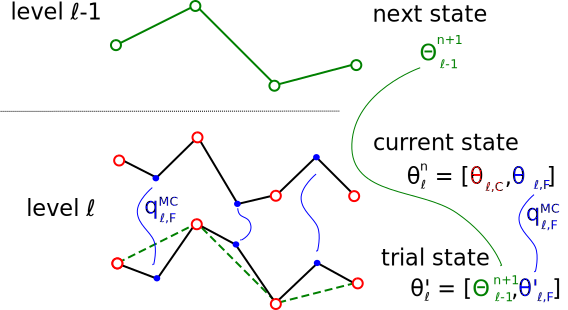
\includegraphics[width=0.7\linewidth]{multilevel_paths.pdf}
  \caption{Multilevel paths}
  \label{fig:multilevel_paths}
\end{center}
\end{figure}
Note that the Metropolis acceptance step guarantees that the samples $\theta_\ell^n$ on level $\ell$ are indeed distributed according to $\pi^\ell$.

Above we assumed that it is possible to sample independently from $\pi^{\ell-1}$. This can be achieved by using the above procedure to create two chains on level $\ell$: (a) the chain $\theta_\ell$ which we will use together with the chain $\Theta_{\ell-1}$ to calculate $\hat{Y}_{\ell,N_\ell}^{MC}$ and (b) another chain $\Theta_{\ell}$, for which we only take every $k$-th sample where $k$ is large compared to the autocorrelation time. To a very good approximation this chain then samples from $\pi^\ell$. The procedure is shown schematically in Fig. \ref{fig:chains} and as the authors of \cite{Dodwell2015} remark, the bias error due to any remaining auto-correlation is small.
\begin{figure}
  \begin{center}
    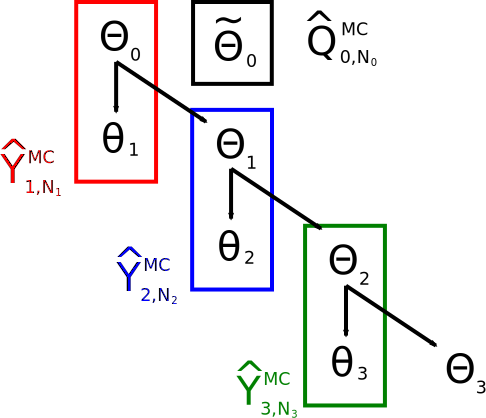
\includegraphics[width=0.3\linewidth]{chains.pdf}
    \caption{Recursive construction of $\theta_\ell$ and $\Theta_\ell$}
    \label{fig:chains}
  \end{center}
\end{figure}
%%%%%%%%%%%%%%%%%%%%%%%%%%%%%%%%%%%%%%%%%%%%%%%%%%%%%%%%%%%%%%%%%%%%%%%%%%%%
\subsubsection{Coarse graining}\label{sec:coarse_graining}
%%%%%%%%%%%%%%%%%%%%%%%%%%%%%%%%%%%%%%%%%%%%%%%%%%%%%%%%%%%%%%%%%%%%%%%%%%%%
To coarse-grain the theory, replace the state vector $\vec{X}=(X_0,X_1,X_2,\dots,X_{M-1})$ by the coarse vector $\vec{X}^{(c)}=(X_0,X_2,X_4,\dots,X_{M/2})$ which only contains the even lattice sites. We now also need to write down a coarse action to define the theory on the coarse lattice. There are two ways of doing this
\begin{itemize}
\item \textit{naive}. Simply take the action in Eq. (\ref{eqn:action}) with $2a$ instead of $a$, i.e.
  \begin{equation}
    S^{(c)}[\vec{X}^{(c)}] = \sum_{j=0}^{M/2} 2a \left(\frac{1}{2}m_0\frac{(X_{2j+1}-X_{2j})^2}{(2a)^2}+V(X_{2j})\right)
    \end{equation}
\item \textit{effective}. Construct the coarse action $S^{(c)}$ such that
  \begin{equation}
    Z^{(c)}[\vec{J}^{(c)}] = \int d^{M/2}\vec{X}^{(c)} \exp\left[-S^{(c)}[\vec{X}^{(c)}]+(\vec{J}^{(c)})^T\vec{X}^{(c)}\right] = Z[\vec{J}^{(c)}]
  \end{equation}
  This results in
  \begin{equation}
    S^{(c)}[\vec{X}^{(c)}] = -\log \left(\int d^{M/2}\vec{X}^{(f)}\; \exp\left[-S[\vec{X}]\right]\right)\qquad\text{where $d^{M/2}\vec{X}^{(f)}=dX_1\;dX_3\;\dots\;dX_{M-1}$}
  \end{equation}
  In other words, the effective action is obtained by integrating out all odd modes $X^{(f)}$ which are not represented on the coarse grid.
\end{itemize}
Note that sampling from the effective action will give coarse level samples which have exactly the same distribution as the coarse modes in a fine level sample.
Calculation of the effective action is only possible in exceptional cases (for example, the harmonic oscillator). In other cases it will be a very complicated object. However, it can be calculated approximately, and will lead to a much better coarse level model than the naive approach which fails to represent fluctuations of size $\sim a$.

For example, consider the quartic oscillator, $V(x) = \frac{1}{2}\mu_0 x^2 + \frac{1}{4}\lambda_0 x^4$. In this case the fine-level and an approximate coarse-grained action would be
\begin{equation}
  \begin{aligned}
  S[\vec{X}] = \sum_{j=0}^{M-1} a \left(\frac{1}{2}m_0\frac{(X_{j+1}-X_{j})^2}{a^2}+\frac{1}{2}\mu_0 X_{j}^2 + \frac{1}{4}\lambda_0 X_{j}^4\right)\\
  S^{(c)}[\vec{X}^{(c)}] = \sum_{j=0}^{M/2-1} 2a \left(\frac{1}{2}m^{(c)}_0\frac{(X_{2j+1}-X_{2j})^2}{(2a)^2}+\frac{1}{2}\mu_0^{(c)}X_{2j}^2 + \frac{1}{4}\lambda_0^{(c)} X_{2j}^4\right)
  \end{aligned}
\end{equation}
where
\begin{xalignat}{3}
  m_0^{(c)} &= m_0^{(c)}(m_0,\mu_0,\lambda_0), &
  \mu_0^{(c)} &= \mu_0^{(c)}(m_0,\mu_0,\lambda_0), &
  \lambda_0^{(c)} &= \lambda_0^{(c)}(m_0,\mu_0,\lambda_0)\label{eqn:renormalised_couplings}
\end{xalignat}
can be calculated using perturbation theory.
%%%%%%%%%%%%%%%%%%%%%%%%%%%%%%%%%%%%%%%%%%%%%%%%%%%%%%%%%%%%%%%%%%%%%%%%%%%%
\subsection{Quantum field theory}\label{sec:QFT}
%%%%%%%%%%%%%%%%%%%%%%%%%%%%%%%%%%%%%%%%%%%%%%%%%%%%%%%%%%%%%%%%%%%%%%%%%%%%
The quantum theory above is one-dimensional, i.e. there is only a lattice in the time-direction. In the continuum a configuration of the system is described by a path $x(t)$. In quantum field theory this is replaced by a field $\phi(\vec{x},t)$ which is a function of the independent space-time variables $\vec{x}\in\mathbb{R}^3$ and $t\in\mathbb{R}$, and hence the theory becomes four-dimensional. However, the same ideas as above apply. The Generating functional is now written as an integral over field configurations
\begin{equation}
Z[J] = \int\mathcal{D}\phi(\vec{x},t)\;\exp\left[-S[\phi(\vec{x},t)]+\int
  J(\vec{x},t)\phi(\vec{x},t)\;d^3\vec{x}\;dt)\right]
\end{equation}
Where the action $S[\phi(\vec{x},t)]$ is an integral over four-dimensional space-time. Discretisation works exactly as above, but now we have a four-dimensional space-time lattice. Coarse-graining by removing lattice sites will be much more effective in four dimensions since the number of points is reduced by a factor 16 instead of 2.
%%%%%%%%%%%%%%%%%%%%%%%%%%%%%%%%%%%%%%%%%%%%%%%%%%%%%%%%%%%%%%%%%%%%%%%%%%%%
\subsubsection{Renormalisation and Effective Theories}
%%%%%%%%%%%%%%%%%%%%%%%%%%%%%%%%%%%%%%%%%%%%%%%%%%%%%%%%%%%%%%%%%%%%%%%%%%%%
One key requirement in Multilevel Monte Carlo calculations is that the ``coarse'' theory is similar to the theory on the finest level. Only in this case the correct variance decay can be guaranteed. In many applications a natural hierarchy exists. For example, if a stochastic differential equation is solved using MLMC, the next coarsest level is simply obtained by halving the time step size, while keeping the other parameters of the system constant.
In QFTs the coarse-graining procedure which halves the lattice spacing corresponds to a renormalisation group transformation, integrating out all fluctations in the energy shell between $1/a$ and $1/(2a)$. The result is an effective theory, which is usually more complicated than the original theory since it contains additional couplings.
However, in some cases only a small set of couplings remain relevant as $a\rightarrow 0$ and the effective theory can be calculated with perturbative methods as long as $a<a_*$. This is the case for QCD, which is an asymptotically free theory. Hence, the idea for the coarse theory construction is to use perturbation theory, and coarsen the theory up to the point where the perturbative expansion breaks down. The critical lattice spacing $a_*$ is a fixed physical parameter, and hence we expect the cost of the MLMCMC calculation to become $\mathcal{O}(\epsilon^{-2}a_*^{-d})=\mathcal{O}(\epsilon^{-2})$ as $\epsilon\rightarrow 0$.
%%%%%%%%%%%%%%%%%%%%%%%%%%%%%%%%%%%%%%%%%%%%%%%%%%%%%%%%%%%%%%%%%%%%%%%%%%%%
\subsubsection{Connections to statistical physics}
%%%%%%%%%%%%%%%%%%%%%%%%%%%%%%%%%%%%%%%%%%%%%%%%%%%%%%%%%%%%%%%%%%%%%%%%%%%%

%%%%%%%%%%%%%%%%%%%%%%%%%%%%%%%%%%%%%%%%%%%%%%%%%%%%%%%%%%%%%%%%%%%%%%%%%%%%
\section{Workplan}
%%%%%%%%%%%%%%%%%%%%%%%%%%%%%%%%%%%%%%%%%%%%%%%%%%%%%%%%%%%%%%%%%%%%%%%%%%%%
Lattice QCD is a highly complicated theory, in particular it contains a non-trivial gauge theory under $SU(3)$ transformations which as to be taken into account during the sampling process. Perturbative calculations of the lattice are also non-trivial. We therefore propose to approach the problem in several stages of increasing complexity:
%%%%%%%%%%%%%%%%%%%%%%%%%%%%%%%%%%%%%%%%%%%%%%%%%%%%%%%%%%%%%%%%%%%%%%%%%%%%
\subsection{Simple quantum mechanical systems}
%%%%%%%%%%%%%%%%%%%%%%%%%%%%%%%%%%%%%%%%%%%%%%%%%%%%%%%%%%%%%%%%%%%%%%%%%%%%
To start with, consider one-dimensional quantum system such as the quadratic or quartic oscillator; an elementary discussion of Monte Carlo sampling for this system can be found in \cite{Creutz1981}. For the quadratic oscillator all integrals are Gaussian and can be solved exactly (including both finite-volume and finite-size effects), which allows comparison to known theory. In this case it is also possible to sample directly (avoiding MCMC), which could lead to further simplifications.
Next, consider the quartic oscillator or a slightly perturbed harmonic oscillator, i.e. systems for which there are no analytical results. The effective action in this case can be calculated with perturbation theory, or one could just use the original action at half the lattice spacing and see what the difference in performance is. The gains in those one-dimensional systems are likely smaller, but could give a guide as to what can be achieved in higher dimensions.
%%%%%%%%%%%%%%%%%%%%%%%%%%%%%%%%%%%%%%%%%%%%%%%%%%%%%%%%%%%%%%%%%%%%%%%%%%%%
\subsection{Quantum Field Theories}
%%%%%%%%%%%%%%%%%%%%%%%%%%%%%%%%%%%%%%%%%%%%%%%%%%%%%%%%%%%%%%%%%%%%%%%%%%%%
Again consider theories of increasing complexity:
\begin{enumerate}
\item \textit{Free scalar field theory of a massive particle}. Again all integrals are Gaussian and can be solved in principle, allowing a comparison to theory. Obviously this case is a but boring since there is no renormalisation
\item \textit{The non-linear sigma model}. Consider this model in $d=2$ dimensions where it is asymptotically free if the number $N_{\text{spin}}$ of spin components is three or more. In higher dimensions there also appears to be a non-trivial critical point, which might be worth studying and this could potentially be analysed asymptotically for $N_{\text{spin}}\gg 1$
  \item \textit{Lattice QCD}. Study full blown QCD, in particular think about the implications of the $SU(3)$ symmetry for Multilevel Monte Carlo sampling
\end{enumerate}
%%%%%%%%%%%%%%%%%%%%%%%%%%%%%%%%%%%%%%%%%%%%%%%%%%%%%%%%%%%%%%%%%%%%%%%%%%%%
\subsection{Code development}
%%%%%%%%%%%%%%%%%%%%%%%%%%%%%%%%%%%%%%%%%%%%%%%%%%%%%%%%%%%%%%%%%%%%%%%%%%%%
Implement the techniques by either developing a bespoke multilevel software for lattice QCD or incorporate it into existing codes such as CHROMA \cite{Edwards2005}. Run code on clusters to obtain calculations of benchmark quantities to higher accuracy. \note{Link to CRAY/GW4 Isambard?}
%%%%%%%%%%%%%%%%%%%%%%%%%%%%%%%%%%%%%%%%%%%%%%%%%%%%%%%%%%%%%%%%%%%%%%%%%%%%
\section{Tasks/Questions}
%%%%%%%%%%%%%%%%%%%%%%%%%%%%%%%%%%%%%%%%%%%%%%%%%%%%%%%%%%%%%%%%%%%%%%%%%%%%
\begin{itemize}
  \item Understand Hybrid Monte Carlo and how it relates to multilevel sampling. For example, does the hierarchical sampling in Multilevel MCMC make Hybrid MC for the suggesting the trial state unnecessary?
  \item Understand the implications of $SU(3)$ invariance for coupling between levels
  \item Renormalisation on the lattice
\end{itemize}
\appendix
%%%%%%%%%%%%%%%%%%%%%%%%%%%%%%%%%%%%%%%%%%%%%%%%%%%%%%%%%%%%%%%%%%%%%%%%%%%%
\section{Harmonic Oscillator}\label{sec:harmonic_oscillator}
%%%%%%%%%%%%%%%%%%%%%%%%%%%%%%%%%%%%%%%%%%%%%%%%%%%%%%%%%%%%%%%%%%%%%%%%%%%%
It is convenient to define a \textit{generating functional}
\begin{equation}
  Z[J] = \int \mathcal{D}x(t)\;\exp\left[-S[x(t)]+\int_0^T J(t)x(t)\;dt \right]\label{eqn:generating_functional_cont}
\end{equation}
where now the sum goes over all paths with periodic boundary conditions $x(0)=x(T)$. This allows extraction of connected $n$-point functions as
\begin{equation}
  \Gamma_c^{(n)} = \frac{\delta}{\delta J(x_1)}\dots\frac{\delta}{\delta J(x_n)} \log\left(Z[J]\right)
\end{equation}
for example
\begin{equation}
  \Gamma_c^{(2)} = \langle x(t_1)x(t_2)\rangle - \langle x(t_1)\rangle \langle x(t_2)\rangle
\end{equation}

Note that for a harmonic oscillator with $V(x) = \frac{1}{2}\mu^2 x^2$ the integral is Gaussian
\begin{equation}
  Z[\vec{J}] = \int d^M\vec{x}\;\exp\left[-\vec{X}^T G \vec{X} + \vec{J}^T \vec{X}\right]
  \end{equation}
with the $M\times M$ correlation matrix
\begin{equation}
  G = \begin{pmatrix}
    a\mu^2 + 2a^{-1} & -a^{-1} & & \dots & & -a^{-1}\\
    -a^{-1} & a\mu^2 + 2a^{-1} & -a^{-1} & &\\
    & -a^{-1} & a\mu^2 + 2a^{-1} & -a^{-1} & & \vdots\\
    \vdots & & & \ddots\\
    & & & -a^{-1} & a\mu^2 + 2a^{-1} & -a^{-1}\\
        -a^{-1} & & \dots & & -a^{-1} & a\mu^2 + 2a^{-1}\\
  \end{pmatrix}
\end{equation}
and hence
\begin{equation}
  \log\left(Z[\vec{J}]\right) = C(a) + \frac{1}{2}\vec{J}^T G^{-1} \vec{J}
\end{equation}
where $C(a)$ is a constant.
This immediately allows the calculation of
\begin{equation}
  \langle X^2\rangle = \langle X_j^2 \rangle = \left(G^{-1}\right)_{jj} = \frac{1}{M}\operatorname{trace}\left(G^{-1}\right) = \sum_{k=0}^{N-1} \left(\mu^2 + \frac{4\sin^2(ka/2)}{a^2}\right)^{-1}
\end{equation}
Upon suitable scaling $\langle X^2\rangle$ is related to the ground state energy. Note that due to translational invariance $\langle X_j^2\rangle =\langle X_0^2\rangle$ and $\left(G^{-1}\right)_{jj}=\left(G^{-1}\right)_{00}=\frac{1}{M}\operatorname{trace}\left(G^{-1}\right)$ for any $j=0,\dots,M-1$.
\bibliographystyle{unsrt}
\bibliography{plan}
\end{document}
